\section{Introduction}
In this project, we investigate how the skills and the age seniorities of $24$ players influence their ranking in competitions. This is done using the results for $134$ games played over $21$ years. Figure~\ref{fig:1} plots the number of games each player has played and the frequency they came first and last. There is a large variation in the number of games participated by each player. Player $10$ takes part in the largest number of games ($=77$) while player $6$ and player $14$ only participate in $2$ games each. Among players who participate in more than $10$ games, player $19$ has the highest $77.8\%$ of coming top among the games played, indicating it is likely to be a strong player, while player $9$ has the highest $87.5\%$ of coming bottom, giving evidence that it is a weak player.
\begin{figure}[ht!]
\centering
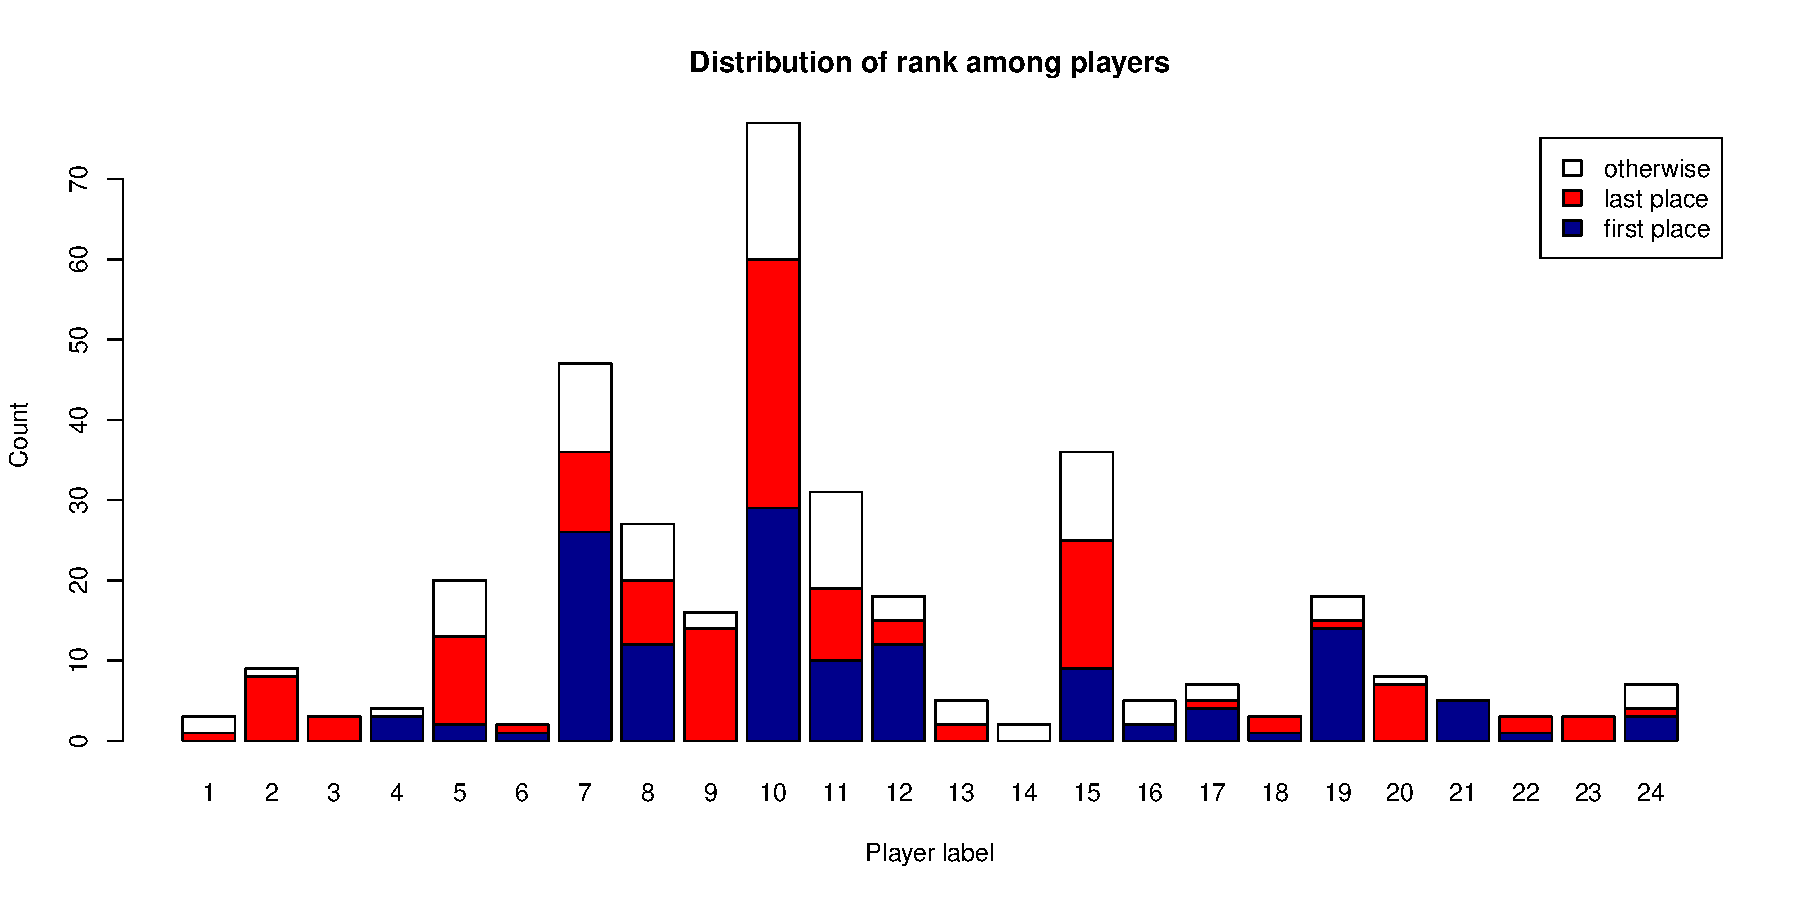
\includegraphics[width=0.9\linewidth]{player}
\caption{The distribution of ranking among the games participated by each of the $24$ players.}
\label{fig:1}
\end{figure}

Figure~\ref{fig:2} plots the fractions of the three seniority levels (1-5, 6-10 and 11-16) among players who are ranked at the top and the bottom place among all $134$ games. From the plot, there is no clear evidence that seniority rank influences the outcomes of the games.
\begin{figure}[ht!]
\centering
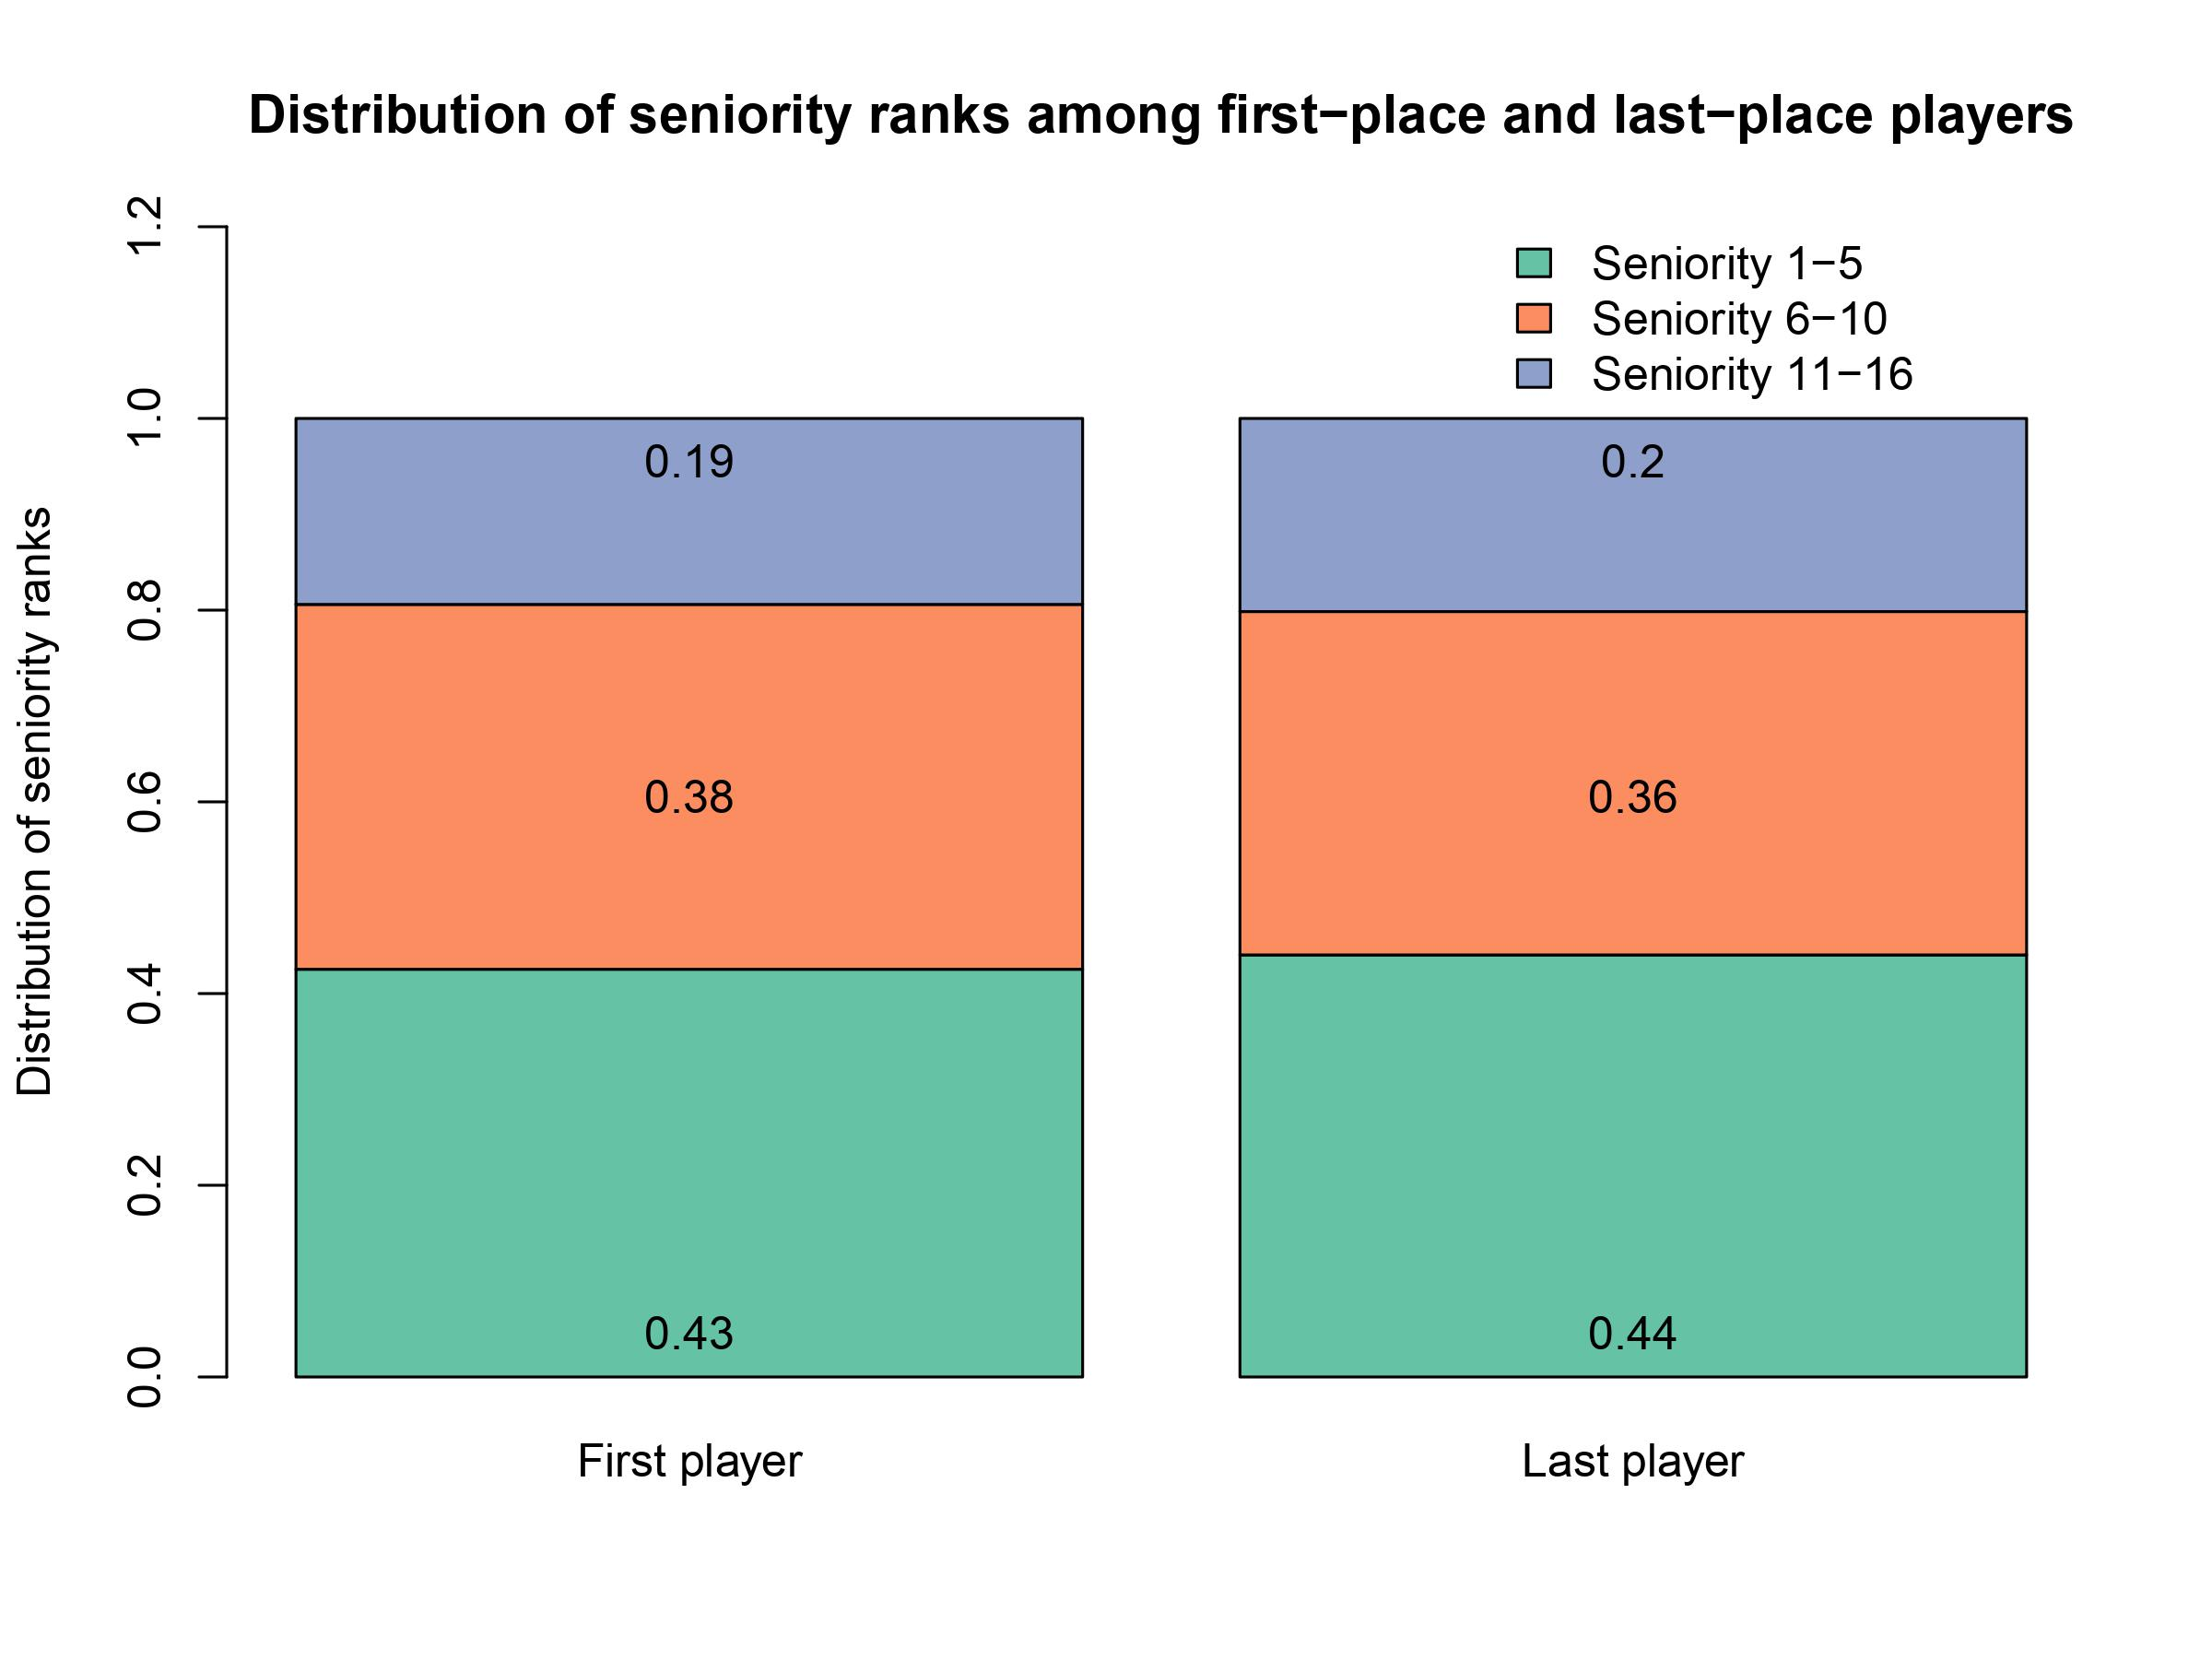
\includegraphics[width=0.65\linewidth]{seniority}
\caption{The distribution of seniority ranks among first-place and last-place players.}
\label{fig:2}
\end{figure}

In the following sections, we will consider two Plackett-Luce observation models, one taking into account the effects of seniority and one without. We will carry out model selection and further test the significance of seniority in determining the game outcomes.
